	
\documentclass[a4paper,12pt]{article}
\usepackage[utf8]{inputenc}

%  Русский язык
\usepackage{multirow}
\usepackage{wrapfig}
\usepackage[T2A]{fontenc}			% кодировка
\usepackage[utf8]{inputenc}			% кодировка исходного текста
\usepackage[english,russian]{babel}	% локализация и переносы

\usepackage{indentfirst} %Красная строка
\usepackage[a4paper,top=1.3cm,bottom=2cm,left=1.5cm,right=1.5cm,marginparwidth=0.5cm]{geometry}
\usepackage[usenames]{color}
\usepackage{colortbl}
\usepackage{csvsimple}
\usepackage{siunitx}

\addto\captionsrussian{\def\refname{5   Список используемой литературы}}

% Заметки
\usepackage{todonotes}

% Математика
\usepackage{amsmath,amsfonts,amssymb,amsthm,mathtools} 
\usepackage{hyperref}

\renewcommand{\AA}{\ensuremath{\mathring{A}}}

\begin{document}
\def\figurename{Рисунок}
\begin{titlepage}
\begin{center}
    {\large МОСКОВСКИЙ ФИЗИКО-ТЕХНИЧЕСКИЙ ИНСТИТУТ (НАЦИОНАЛЬНЫЙ ИССЛЕДОВАТЕЛЬСКИЙ УНИВЕРСИТЕТ)}
\end{center}
\begin{center}
    {\largeФизтех-школа биологической и медицинской физики}
\end{center}

\vspace{1cm}
{\huge
\begin{center}
    {\bf Лабораторная работа по физической химии}\\
    \vspace{0.5cm}
   Образование, устойчивость и свойства лиофобных коллоидных растворов.
\end{center}
}

\vspace{4cm}
\begin{flushright}
{\LARGE Выполнила студентка группы Б06-103:\\ Фитэль Алена \\}

\end{flushright}
\vspace{9cm}
\begin{center}
    Долгопрудный, 2023 г.
\end{center}
\end{titlepage}
\newpage

\section{Введение}
\setcounter{page}{2}
\textbf{Цели работы}: 
\begin{itemize}
 \item Получение лиофобных коллоидных растворов и исследование их свойств
    \item Для золя золота определить размер частиц 
    \item Определить порог коагуляции отрицательно заряженного золя золота по отношению к различным электролитам и определить механизм его коагуляции
\end{itemize}
\section{Теоретическая справка \cite{1}}
\subsection{Типы коллоидных растворов}
Согласно классификации П.А.Ребиндера коллоидные растворы подразделяются на:

Лиофильные —  большое сродство к растворителю, термодинамически устойчивы к агрегации и образуются самопроизвольно. Низкое значение поверхностного натяжения.

Лиофобные — термодинамически неустойчивы к агрегации, образуются несамопроизвольно в результате диспергирования или конденсации с пересыщением. Могут быть устойчивы кинетически. Обладают избытком поверхностной энергии.

\subsection{Методы получения лиофобных коллоидных растворов}

Пептизация - процесс перехода осадка в коллоидный раствор, то есть из состояния агрегатов мы получаем маленькие коллоидные частички. Процесс происходит при добавлении пептизатора, который адсорбируется на поверхности, дает заряд, так что частицы начинают отталкиваться и осадок диспергирует. 

Конденсация - создание коллоидного раствора из молекулярного. Например из истинного при замене растворителя. В нашей работе это показано на примере получения золя серы. Если капнуть в воду ацетон с растворенной в нем серой, то , попав в полярный растворитель, неполярная сера уже не будет растворяться и начнется конденсация.

\subsection{Термодинамические факторы стабилизации коллоидных систем}

Как мы знаем, лиофобные коллоидные расторы сами по себе не образуются и неустойчивы термодинамически. Но можно их стабилизировать. 

Стабилизация возможна засчет снижения поверхностного натяжения между частицами и раствором. Это важно, ведь когда идет дисперегирование, то происходит увеличение суммарной площади контакта растрителя и частиц, а для энергии эта площадь умножаестя на межфазное натяжение. 

Также можно заставить некоторые ионы специфически адсорбироаться на частицах и у них появится заряд. Это электростатический фактор стабилизации. Можно отемтить, что в этом случае заряд частиц не только отталкивает их. Также они притягивавет к частице молекулы расторителя и снижается поверхностное натяжение.

\subsection{Кинетическая устойчивость лиофобных коллоидов}
Устойчивость определяется скоростью процесса коагуляции, который можно описать с помощью уравнения Смолуховского: 
\begin{equation}
    \nu_{\tau} = \frac{\nu_{0}}{1+K \cdot \nu_{0}}
\end{equation}
Константа скорости коагуляции определяется потенциальным барьером при взаимодействии частиц с  энергией активации $\Delta E$  и стерическим фактором $P$, зависит от вязкости растворителя $\eta$:
\begin{equation}
    K = \frac{4kT}{3 \eta} P\cdot \exp  \left(-\frac{\Delta E}{kT} \right)
\end{equation}
В целом константа скорости K определяет медленную коагуляцию (при достаточно высоком активационном барьере скорость агрегации может сравнятся со скоростью диспергирования и система окажется устойчивой к коагуляции). Первая дробь определяет быструю коагуляцию (потенциальный барьер отсутствует)

\subsection{Энергия взаимодействия между частицами в коллоидном растворе}
Частицы фазы заряжены, поэтому они взаимодействуют друг с другом.

Энергия притяжения — силы Ван-дер-Ваальса $ \sim \frac{1}{r^2}$ 

Энергия отталкивания, согласно теории ДЛФО (Дерягина-Ландау-Фервея-Овербека) сила  отталкивания  частиц  имеет 
электростатическую  природу  (так  называемое  расклинивающее  давление) $ \sim \frac{1}{e^r}$ 

\begin{figure}[h!]
    \centering
    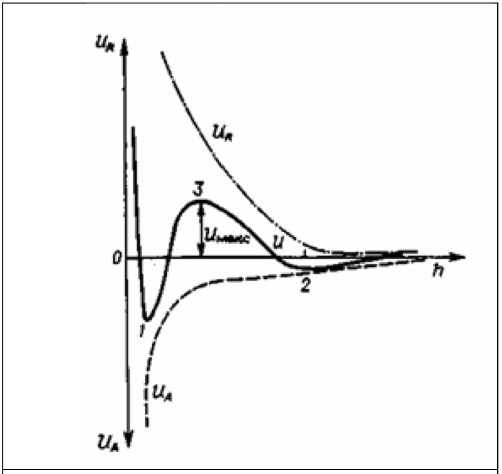
\includegraphics[scale = 0.4]{Screenshot 2023-02-13 at 8.56.28 PM.png}
    \caption{Зависимость энергии взаимодействия U двух частиц от расстояния h между ними. Цифрами отмечены: 1 - минимум энергии при  непосредственном контакте двух частиц; 2 - минимум энергии при дисперсионном притяжении на сравнительно больших расстояниях; 3 – потенциальный барьер. }
    \label{fig : 1}
\end{figure}

Верхняя прерывистая кривая отвечает электростатичекой энергии отталкивания, 
нижняя - притяжения за счет сил Ван-дер- 
Ваальса. Сплошная кривая отвечает  их  суперпозиции.  

Введение электролитов снижает величину потенциального барьера благодаря увеличению крутизны верхней кривой для электростатической энергии отталкивания (сжатию двойного слоя), либо уменьшению ее амплитуды (нейтрализация заряда частицы).

Одним из наиболее известных способов коагуляции лиофобных систем является действие растворов электролитов. Различают два типа электролитной коагуляции:
\begin{enumerate}
    \item Нейтрализационная — ионы электролита адсорбируются на коллоидной частице, понижая при этом ее заряд; отталкивание между частицами уменьшается, следовательно понижается энергетический барьер и частицы начинают лучше коагулировать
    \item Концентрационная — коллоидная частица окружена диффузным ДЭС, толщина которого зависит от ионной силы раствора 
    \begin{equation}
        I=\frac{1}{2}\sum c_i\cdot z_{i}^2
    \end{equation}
    следующим образом (согласно теории Гуи-Чапмена) 
    \begin{equation}
        \lambda = \sqrt{\frac{\epsilon \epsilon_0 RT}{2 F^2 I}}
    \end{equation}
    При добавлении электролита увеличивается ионная сила раствора (с ростом концентрации многозарядных ионов) и уменьшается толщина диффузного слоя ДЭС, это позволяет частицам ближе подойти друг к другу и коагулировать, (эффективнее проводить при высоких поверхностных зарядах)
\end{enumerate}

Концентрация электролита, при которой энергетический барьер исчезает, называется порогом быстрой коагуляции 
\begin{equation}
    C_{пк} = \frac{C_{э} V_{э}}{V_{э}+V_{золь}}
\end{equation}

Отличаются два типа электролитной коагуляции правилами, которые применяются в этих случаях:

Коагулирующим действием обладает ион со знаком, противоположным поверхности, 

но для концетрационного механизма по \textbf{правилу Дерягина-Ландау} коагулирующее действие зависит от заряда противоиона как $ \sim \frac{1}{z^6}$. 

а для нейтрализационного механизма зависимость по \textbf{правилу Эйлерса-Корфа} имеет вид $ \sim \frac{1}{z^2}$.
\subsection{Строение двойного электрического слоя.}

Ионы, которые избирательно адсорбируются на коллоидной частице, создают $\phi$-потенциал. Ионы, создающие такой потенциал, называются потенциалопределяющими. На практике его определить практически невозможно, однако есть другой метод оценки заряда и потенциала коллоидных частиц — определение скорости их движения в электрическом поле. 

В процессе такого движения ДЭС разрывается, место разрыва называется плоскостью скольжения (располагается на границе между диффузным и плотным слоями). Потенциал на плоскости скольжения называют электрокинетическим или $\zeta$-потенциалом (это разность потенциалов дисперсионной среды и неподвижного слоя жидкости, окружающего частицу). Важно, что его значение может быть связано с устойчивостью коллоидов (при ǀ$\zeta$ǀ>30 мВ коллоид считается устойчивым)

\textbf{Правила избирательной адсорбции:}
\begin{enumerate}
    \item В растворе с ионами одинаковой концентрации легче адсорбируются ионы с большим зарядом
    \item В растворе с ионами одинакового заряда легче адсорбируются ионы, которые представлены в большей концентрации
    \item В растворе с ионами, чьи заряды и концентрации равны лучше адсорбируются те, которые могут достраивать кристаллическую решетку или образуют труднорастворимое соединение с ионами, составляющими кристаллическую решетку (по правилу Фаянса-Пескова-Панета)
    \item Хорошо адсорбируются ионы, которые сильнее деформируются под действием электрического поля решетки (тем самым уменьшая полярность связи)
    \item Из ионов с одинаковым зарядом лучше адсорбируются менее гидратированные ионы (адсорбционного способность нарастает в лиотропных рядах Гоффмейстера)
\end{enumerate}
\subsection{Строение коллоидной мицеллы.}

Совокупность коллоидных частиц в центре мицеллы — агрегат. Ядро мицеллы составляют агрегат и потенциалопределяющие ионы. На поверхности ядра образуется ДЭС, подобный электрическому 
конденсатору и аналогичный такому же слою у поверхности заряженных металлических 
электродов. 

\begin{figure}[h!]
    \centering
    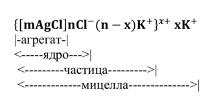
\includegraphics[scale = 1]{image.jpeg}
    \caption{Строение мицеллы (формула золя)}
    \label{fig : 2}
\end{figure}

\subsection{Кинетика коагуляции}

Наши приближения: 1) слипание происходит при броунировании 2) все частицы сферичны и одного диаметра 3) коагуляция быстрая ($E_A = 0$) 4) а каждом акте участвуют только 2 частицы. Тогда оценим время полукоагуляции:

\begin{figure}[h!]
    \centering
    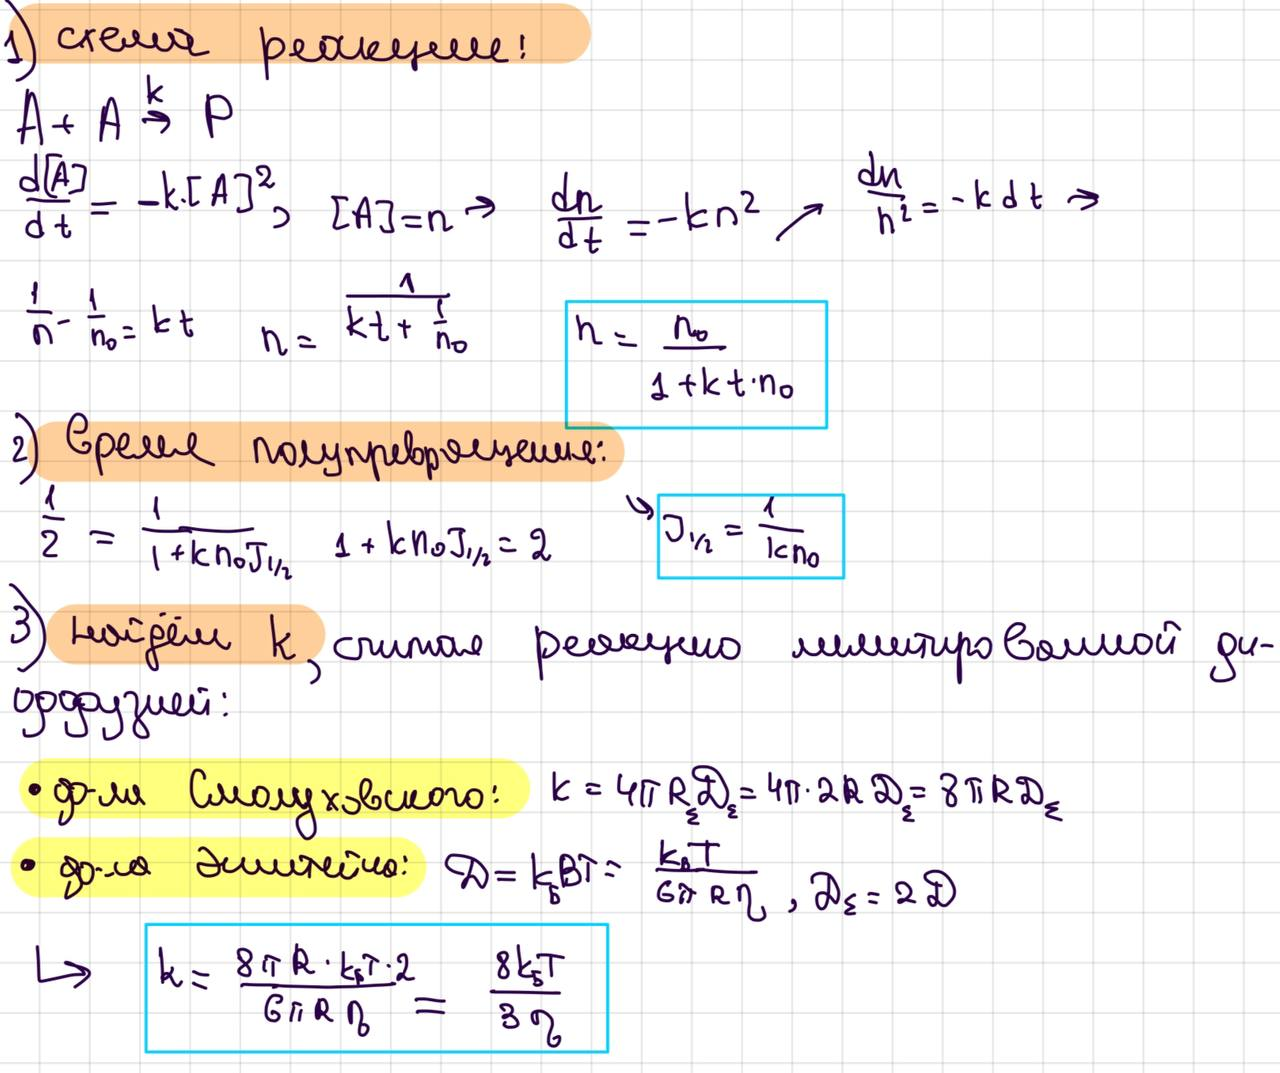
\includegraphics[scale = 0.25]{calc.jpg}
    \caption{Вывод формулы для расчета времени полупревращения.}
    \label{fig : 1}
\end{figure}


 
\newpage
\section{Практическая часть}
\subsection{ Получение золей и исследование их свойств}
\subsubsection{Получение золя серы S методом замены растворителя}
Нальем в пробирку 5-6 мл дистиллированной воды и добавим туда несколько капель отфильтрованного насыщенного раствора серы в ацетоне. 

Через 1 минуту раствор стал коллоидным и начал опалесцировать: менять свой цвет с оранжевого в проходящем свете на голубой в рассеянном.

\subsubsection{Получение золя гидроксида железа $Fe(OH)_3$ методом конденсации}
\begin{enumerate}
    \item В стакан из термостойкого стекла нальем 50 мл дистиллированной воды. Нагреем воду на электроплитке с магнитной мешалкой до кипения. Не снимая колбы с электроплитки, медленно, при перемешивании вольем в воду 5 мл 2\%-ного раствора $FeCl_3$.
    \item В результате реакции образовался раствора коньячного цвета: 

\[FeCl_3 + 3H_2O = Fe(OH)_3 \downarrow+3HCl\]

Стабилизатором реакции является оксохлорид железа, образующийся в результате:

\[Fe(OH)_3 + 3HCl = FeOCl + 2H_2O\]

\[FeOCl=FeO^{+}+Cl^{-}\]

\item  Объясним избирательную адсорбцию катионов на поверхности $Fe(OH)_3$. В растворе присутствуют ионы: $FeO^{+}$,$Cl^{ -}$,$Fe^{3+}$, $OH^{-}$. В результате гидролиза среда в растворе кислая, поэтому $OH^{-}$ не могли достраивать кристаллическую решетку. Так как гидролиз происходил при нагревании, то равновесие смещено в сторону продуктов реакции, значит концентрация $Fe^{3+}$ мала. Согласно правилу Фаянса-Пескова-Панета, лучше адсорбироваться на поверхности  $Fe(OH)_3$ будут ионы $FeO^{+}$ или $Fe^{3+}$, т.к. они могут достраивать кристаллическую решетку. Концентрация $Fe^{3+}$ мала, значит преимущественно будет образовываться мицеллы
$[[mFe(OH)_3]n FeO^{+} (n-x) Cl^{-}]^{x+} xCl^{-}$, и в меньшей степени $[[mFe(OH)_3]n Fe^{+3} (3n-x) Cl^{-}]^{x+} xCl^{-}$ . 


\end{enumerate}
 

\subsubsection{Получение золя гидроксида железа $Fe(OH)_3$ методом пептизации}
\begin{enumerate}
    \item В стакан нальем 25 мл дистиллированной воды и 0,5 мл 10\%-ного раствора $FeCl_3$. К полученному раствору добавим по каплям 10\%-ный раствор аммиака до тех пор, пока количество образующегося осадка не перестанет увеличиваться. 
    \item В стакане идет реакция образования осадка гидроксида железа:
    \[FeCl_3+3NH_3H_2O=Fe(OH)_3\downarrow+3NH_4Cl\]
    \item Даем осадку полностью осесть и аккуратно декантируем, т. е. осторожно сливаем раствор над осадком в стакан, следя за тем, чтобы осадок оставался на месте. Добавляем к осадку приблизительно 30 мл дистиллированной воды, взбалтываем, даем отстояться и снова декантируем. Повторяем такую же промывку и декантацию ещё два раза. 
    \item К промытому осадку добавляем 25 мл дистиллированной воды, взбалтываем и, не давая гидроксиду железа осесть, переносим пипеткой по 2 мл образовавшейся суспензии в 5 чистых пробирок, находящихся в штативе.
\item Добавим в каждую пробирку указанные в таблице объёмы дистиллированной воды и пептизатора (10\%-ного раствора $FeCl_3$). Энергично перемешаем содержимое всех пробирок и оставим их в штативе на 1 час. По истечении часа сравним объёмы осадков в пробирках с пептизатором и в контрольной пробирке (№1). Результаты пептизации растворов приведены в Таблице 1, на Рисунке 3 изображена фотография растворов по истечению часа.

\begin{table}[h!]
\centering
\caption{Степень пептизации $Fe(OH)_3$ растворов с разным количеством пептизатора.}
\begin{tabular}{|c|c|c|c|c|c|}
\hline
№ пробирок           & 1 & 2   & 3   & 4   & 5    \\ \hline
Объём суспензии $Fe(OH)_3$, мл & 2 & 2   & 2   & 2   & 2    \\ \hline
Объём воды, мл       & 5 & 4,8 & 4,6 & 4,4 & 4,2  \\ \hline
Объём 10\%-ного $FeCl_3$, мл & - & 0,2 & 0,4 & 0,6 & 0,8  \\ \hline
Степень пептизации   & - & +   & ++  & +++ & ++++ \\ \hline
\end{tabular}
\end{table}


\begin{figure}[h!]
    \centering
    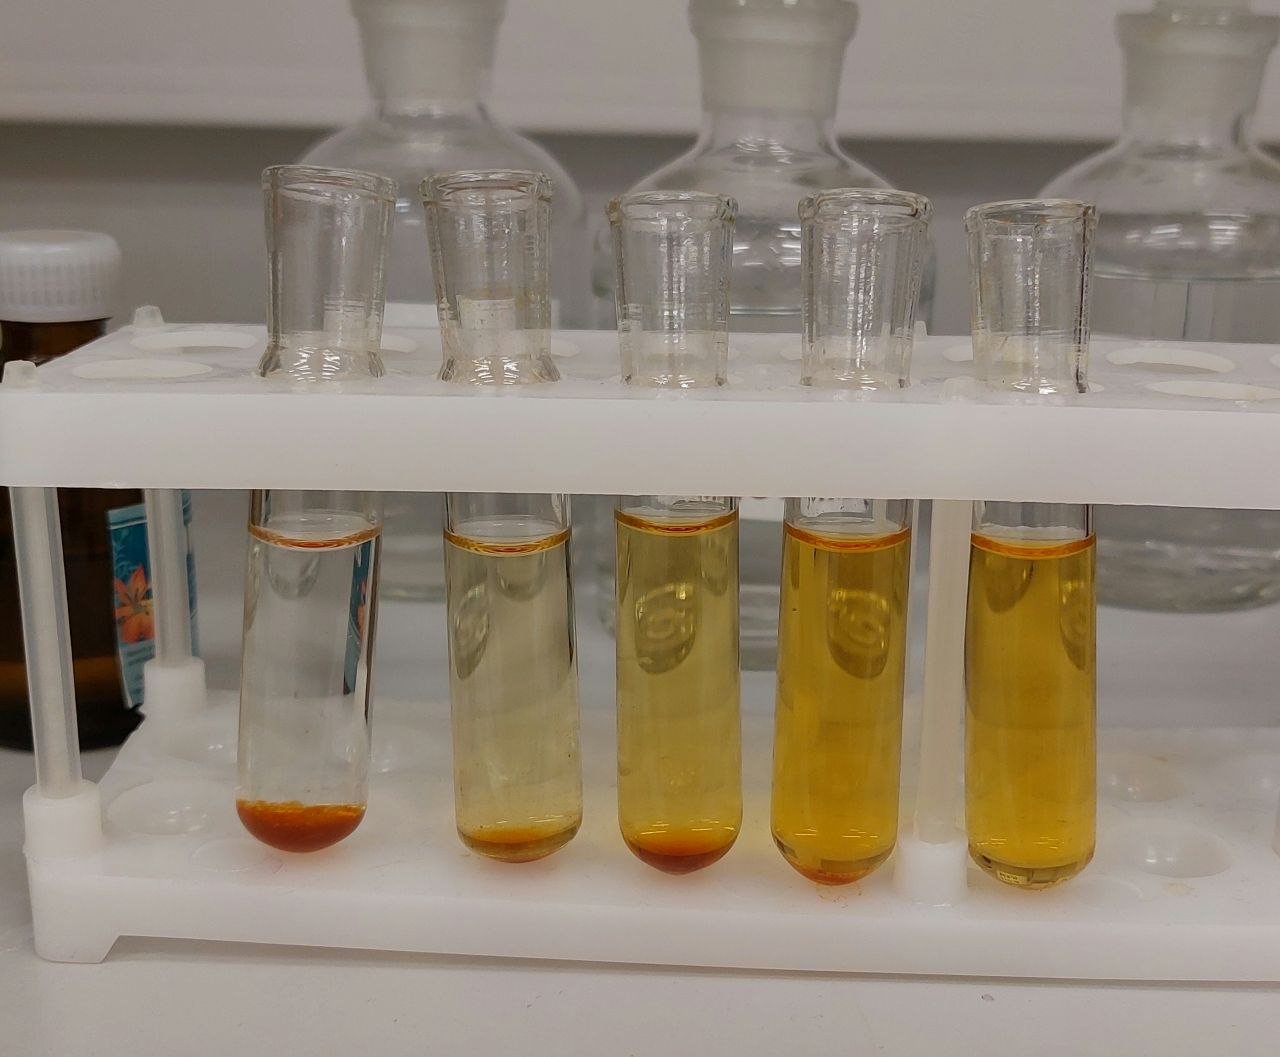
\includegraphics[scale = 0.25]{kold.jpg}
    \caption{Степень пептизации растворов с разным количеством пептизатора.}
    \label{fig : 1}
\end{figure}

\item Схема процесса, идущего при пептизации и формула образующегося положительно заряженного золя: 
\[mFe(OH)_3+nFeCl_3 \xrightarrow{}[[mFe(OH)_3]nFe^{3+} (3n-x)Cl^{-}]^{x}xCL^{-}\]
\item В растворе присутствуют ионы: $NH_4^{+}$,$Cl^{-}$,$Fe^{3+}$, $OH^{-}$. Согласно правилу Фаянса-Пескова-Панета, лучше адсорбироваться на поверхности  $Fe(OH)_3$ будут ионы  $Fe^{3+}$ либо $OH^{-}$ , т.к. они могут достраивать кристаллическую решетку. Вследствие гидролиза среда раствора кислая, поэтому достраивать решетку будут ионы $Fe^{3+}$, которые к тому же обладают большим по модулю зарядом. Необходимое количество пептизатора $FeCl_3$ для полного перевода полученного осадка $Fe(OH)_3$ в коллоидное состояние: 0.8 мл.

\end{enumerate}



\subsubsection{Отрицательно заряженный золь золота}

\begin{enumerate}
    \item В нагретую до кипения дистиллированную воду (50 мл) добавим 0.15 мл 1 \% раствора золотохлористоводородной кислоты $HAuCl_4$, через три минуты кипячения при размешивании быстро добавим порцию 1 \% раствора цитрата натрия $Na_3Cit$ объемом 3 мл. Затем при размешивании прокипятим смесь 6 минут до тех пор, пока окраска раствора не перестанет меняться. Полученный золь охладим до температуры $\approx 40^{\circ} C$ и будем использовать в последующих опытах.
    
    \item Суммарная реакция цитратного восстановления:

\begin{figure}[h!]
    \centering
    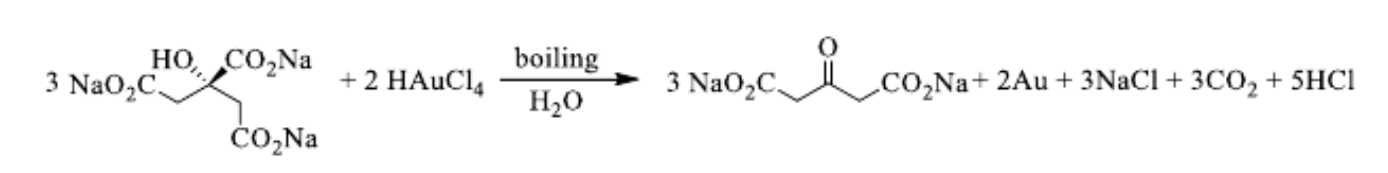
\includegraphics[scale = 0.35]{react.png}
\end{figure}

    \item Определим, какой из реагентов взят в избытке:
\begin{itemize}
    \item $HAuCl_4$: 1\% (по массе) раствор, объем раствора V = 0.15 мл, следовательно $m(HAuCl_4) = 0.01 * 0.15 г = 1,5*10^{-3}$~г, $\nu(HAuCl_4) = \frac{m(HAuCl_4 )}{\mu(HAuCl_4)}=\frac{1,5*10^{-3}г}{340 г/моль}= 4.4 \cdot 10^{-6}$~моль.
    \item $Na_3Cit$: 1\% (по массе) раствор, объем раствора V=1 мл, следовательно  $m(Na_3Cit) = 0.01*1 г=1*10^{-2}$~г, $\nu(Na_3 Cit) =  \frac{m(Na_3Cit)}{\mu(Na_3 Cit)} =\frac{1*10^{-2}  \text{г} }{258 \text{г/моль}}= 39\cdot 10^{-6}$ ~моль.
\end{itemize}

Исходя из стехиометрии, должно быть: $\frac{\nu(HAuCl_4 )}{\nu(Na_3 Cit)}=  \frac{2}{3}$.
Значит, $Na_3Cit$ взят в избытке -  его в 9 раз больше чем $HAuCl_4$,  а не в полтора.
    \item  Из-за избытка $Na_3Cit$, в растворе присутствуют ионы $Na^{+}$,$Cit^{3-}$,из которых большей способностью к адсорбции обладают ионы  $Cit^{3-}$, имеющие больший заряд. Тогда строение заряженной мицеллы золота:
$[[mAu]nCit^{3-} (3n-x) Na^{+}]^{x-} xNa^{+}$.
   
\item Рассчитаем концентрацию золота в получившемся золе.
Исходя из стехиометрии, $\nu(HAuCl_4)=\nu(Au)=4.4*10^{-6}$~моль.
Объем итогового раствора: V=50+0.15+1=51.15 мл. Тогда:

$C(Au)=\frac{\nu(Au)}{V}=\frac{4.4*10^{-6}  моль}{51.15*10^{-3} л}  =8.63\cdot10^{-5}$ ~  моль/л.


\end{enumerate}  


\subsubsection{Определение размера частиц золя золота}

По положению максимума в спектре поглощения золя определим размер частиц золя $Au$.
\begin{itemize}
    \item Зависимость между максимумом спектра поглощения $\lambda_{max}$ и диаметром коллоидных частиц $d$ \cite{2} :
\begin{equation}
    \lambda_{max} = 518.8-0.0172\cdot d+0.0063\cdot d^2-0.0000134*d^3
\end{equation}
\item Из показаний спектрофотометра (Рисунок 4)  определим максимум поглащения и по зависимости (12) расчитаем диаметр коллоидных частиц: $\lambda_{max} = 523$~нм , значит $d$ = 28.12 нм.
\begin{figure}[h!]
    \centering
    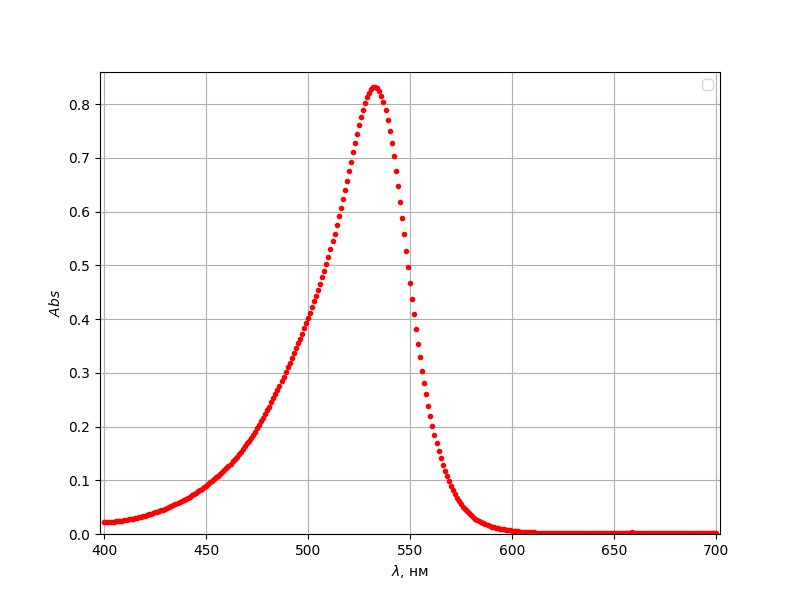
\includegraphics[scale = 0.5]{rrrr.png}
    \caption{Спектр поглащения раствора золя золота.}
    \label{fig : 1}
\end{figure}



\end{itemize}





Рассчитаем количество частиц золя в объеме раствора:
$N=\frac{m}{m_1}$   ,где $m$ - масса частиц в растворе,$m_1$ - масса одной частицы:

\[C(Au)=\frac{\nu(Au)}{V}=\frac{m(Au)}{\mu(Au)\cdot V}\]

\[m = C(Au)\cdot \mu(Au)\cdot V = 8.63\cdot10^{-5} \text{ моль/л} \cdot 197 \text{ г/моль} \cdot 51.15\cdot 10^{-3} \text{ л} = 8.70 \cdot 10^{-4}\text{ г}\]

\[m_1=\rho(Au) \cdot V_1 = \rho(Au) \cdot \frac{4}{3} \pi \cdot \left( \frac{d}{2} \right)^3 = 19.32 \cdot 10^{6} \cdot \frac{4}{3} \pi (\frac{28.12\cdot10^{-9}}{2})^3 = 2.25 \cdot 10^{-16}\text{ г}. \]

Тогда:
$N=\frac{m}{m_1} =\frac{8.70 \cdot 10^{-4} \text{ г}}{2.25 \cdot 10^{-16}  \text{ г}} = 3.87 \cdot 10^{12}$ штук.

\subsection{Определение порогов коагуляции золей}
\begin{enumerate}
    \item Оценим время полупревращения быстрой коагуляции (п. 2.8). В нашем случае( $T = 298 K$,  $\eta(T) = 0.900\cdot 10^{-3} \text{Па с}$ \cite{3}, $N_0 = 6.13 \cdot 10^{11} \text{ штук}$, $V_0 = 51.15 \text{ мл}$, $V_1 = 1 \text{ мл} $ $V_2 = 3 \text{ мл} $ ):

    
    \[ k = \frac{8k_{b}T}{3\eta} = 1.22 \cdot 10^{-17} \frac{\text{м}^{3}} {\text{с}} = 1.22 \cdot 10^{-14} \frac{\text{л}} {\text{с}}\]
    \[
N_1 = \frac{N_0 V_1}{V_0} = 7.57 \cdot 10^{10}\text{ штук} 
    \]
    
    \[n_0 = \frac{N_1}{V_2} = 2.52 \cdot 10^{13}\frac{\text{ штук}}{\text{ л}}\]
   
    \[\tau_{1/2} = \frac{1}{n_0 k} = 3 \text{ с}  
    \]
    
    \item Будем определять пороги коагуляции отрицательно заряженного золя золота по отношению к электролитам, проявляющим различную силу коагуляции в зависимости от зарядов составляющих их ионов. Рассмотрим растворы электролитов: $KNO_3$,$Mg(NO_3)_2$,$La(NO_3)_3$.
    \item Определим для каждой из них порог быстрой коагуляции следующим методом: наливаем в пробирку 2 мл раствора электролита разной концентрации ( изначально, например, по 1 мл воды и электролита) и 1 мл раствора золя золота. По изменению цвета определяем - прошла коагуляция или нет.
    \item В зависимости от результата выбираем следующую нужную концентрацию электролита, придерживаясь метода бинарного поиска ( всего 4-5 раз), пока не определим порог коагуляции. Результаты приведены в Таблице 2. 

\begin{table}[h!]
\centering
\begin{tabular}{|c|c|c|c|c|}
\hline
Электролит             & $c_{\text{э}}$, М          & $V_{\text{в}}$, мл & $V_{\text{э}} $, мл & Коагуляция \\ \hline
$KNO_3 $               & 0.5                   & 0             & 2              & +          \\ \cline{3-5} 
\multicolumn{1}{|l|}{} &                       & 1             & 1              & +          \\ \cline{3-5} 
                       &                       & 1.5           & 0.5            & +          \\ \cline{3-5} 
                       &                       & 1.75          & 0.25           & +          \\ \cline{3-5} 
                       &                       & 1.875         & 0.125          & -          \\ \cline{3-5} 
                       &                       & 1.810         & 0.190          & +          \\ \hline
$Mg(NO3)_2$            & 0.01                  & 0             & 2              & +          \\ \hline
\multicolumn{1}{|l|}{} &                       & 1             & 1              & +          \\ \cline{3-5} 
                       &                       & 1.5           & 0.5            & +          \\ \cline{3-5} 
                       &                       & 1.75          & 0.25           & -          \\ \cline{3-5} 
\multicolumn{1}{|l|}{} & \multicolumn{1}{l|}{} & 1.625         & 0.375          & -          \\ \hline
$La(NO3)_3$            & 0.001                 & 0             & 2              & +          \\ \hline
\multicolumn{1}{|l|}{} &                       & 1             & 1              & +          \\ \cline{3-5} 
                       &                       & 1.5           & 0.5            & -          \\ \cline{3-5} 
                       &                       & 1.25          & 0.75           & -          \\ \cline{3-5} 
                       &                       & 1.125         & 0.875          & -          \\ \hline
\end{tabular}
\caption{Результаты измерений для определения порога коагуляции золя золота}
\label{tab:my-table}
\end{table}
    
    
    
    \item Из результатов измерений найдем порог быстрой коагуляции и определим степень зависимости порога коагуляции от заряда иона. Пусть $C_{\text{ПК}} = \frac{a}{z^{k}}$   где $a,k$ - некоторые константы.  Тогда:
\[\ln (C_{\text{ПК}}) = \ln(\text{ПК})=  \ln(a) - k\ln(z) \hspace{1 cm}  C_\text{ПК} = \frac{V_{\text{э}} \cdot C_{\text{э}}}{V_{0}}, V_0 = 3 \text { мл}
\]


    \item Результаты расчетов порогов коагуляции приведены в Таблице 3. График полученной зависимости изображен на Рисунке 6. По полученному углу наклона имеем: $k = -6.1$,  следовательно $C_{ПК} = \frac{a}{z^{6}}$.


\begin{table}[h!]
\centering
\begin{tabular}{|c|c|l|c|c|}
\hline
z & $\ln{z}$ & $V_{\text{э}} $, мл & $C_{ПК}~, M \cdot 10^{-4}$ & $\ln{C_{ПК}}$ \\ \hline
1 & 0,000    & 0.190               & 316.667                    & -3,452        \\ \hline
2 & 0,693    & 0.381               & 12.700                     & -6.669        \\ \hline
3 & 1,098    & 0.938               & 0.317                      & -10.359       \\ \hline
\end{tabular}
\caption{Пороги быстрой коагуляции.}
\label{tab:my-table}
\end{table}

\begin{figure}[h!]
    \centering
    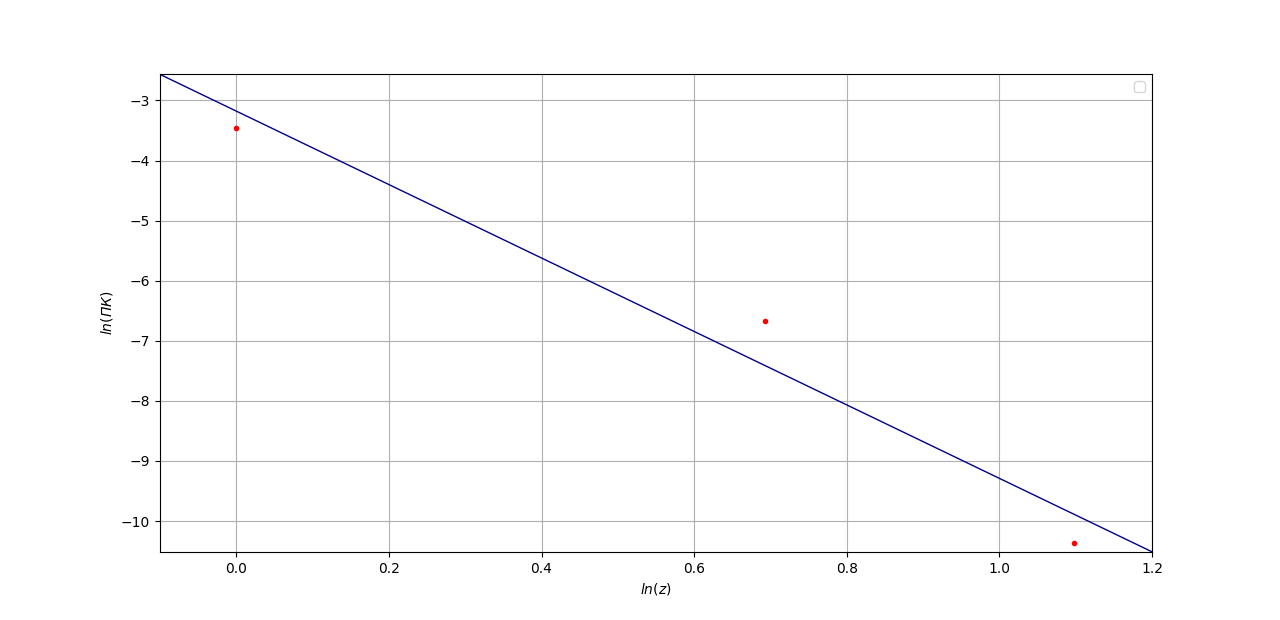
\includegraphics[scale = 0.42]{frr.png}
    \caption{График зависимости порогов коагуляции от заряда электролита.}
    \label{fig : 1}
\end{figure}

\end{enumerate}
\newpage





\section{Обсуждение полученных результатов и выводы}
\begin{itemize}
    \item В ходе работы был получен золь серы методом замены растворителя, гидроксида железа методом конденсации и пептизации. 
    \item Использованием методики Дж. Туркевича был получен золь золота реакцией цитратного восстановления. С помощью спектрофотометрии был оценен размер коллоидных частиц и их число в полученном растворе : $N = 3.87 \cdot 10^{12}$ штук, $d$ = 28.12 нм. 
    \item Для золя золота была проведена оценка времени полукоагуляции: $\tau_{1/2} = 3$ c. Методом бинарного поиска был проведен поиск порогов коагуляции золя в растворе электролитов с различными зарядовыми числами катионов. По итогу измерений был построен график в логарифмических координатах зависимости порога концентрации от зарядового числа. По угла наклона была определена степень зависимости между $C_{\text{ПК}}$ и $z$: $C_{\text{ПК}} \sim z^{6}$, что согласуется с правилом Дерягина - Ландау для концентрационной коагуляции.
    
\end{itemize}

\newpage

\addcontentsline{toc}{section}{Список используемой литературы}
\begin{thebibliography}{}
    \bibitem{1}  Департамент химии МФТИ -  "Образование, устойчивость и свойства лиофобных коллоидных растворов "
    \bibitem{2}  J. Phys. Chem. C 2007, 111, 40, 14664–14669 - "Size Correlation of Optical and Spectroscopic Properties for Gold Nanoparticles"
    \bibitem{3} Расчет вязкости воды 
 для заданной температуры - https://www.freechemistry.ru/sprav/vis-h2o.htm
\end{thebibliography}



\end{document}
\end{document}
